\begin{frame}[fragile]{Tutorial: One-site state basics}

\begin{columns}

\begin{column}[T]{0.48\textwidth}
\begin{onlyenv}<1->
\begin{lstlisting}[language=JuliaLocal, style=julia, basicstyle=\scriptsize\ttfamily]
using ITensors

i = Index(2)

 \end{lstlisting}
\end{onlyenv}
\end{column}

\begin{column}[T]{0.48\textwidth}

\begin{onlyenv}<1-1>
Load ITensor \\[\baselineskip]
2-dimensional labeled \\
Hilbert space \\
(dim=2|id=510)
\end{onlyenv}

\begin{onlyenv}<2->
\begin{figure}[T]
  
\includegraphics[width=0.3\textwidth]{
    slides/assets/i.png
  }
\end{figure}
\end{onlyenv}

\end{column}


\end{columns}

\begin{columns}

\begin{column}[T]{0.48\textwidth}
\begin{onlyenv}<3->
\begin{lstlisting}[language=JuliaLocal, style=julia, basicstyle=\scriptsize\ttfamily]
Zp = ITensor(i)
Zp[i=>1] = 1

Zp = ITensor([1, 0], i)
\end{lstlisting}
\end{onlyenv}
\end{column}

\begin{column}[T]{0.48\textwidth}
\begin{onlyenv}<3-3>
$|Z+\rangle = \begin{bmatrix} 1 \\ 0 \end{bmatrix}$ \\[\baselineskip]
Construct from a Vector
\end{onlyenv}
\begin{onlyenv}<4>
\begin{center}
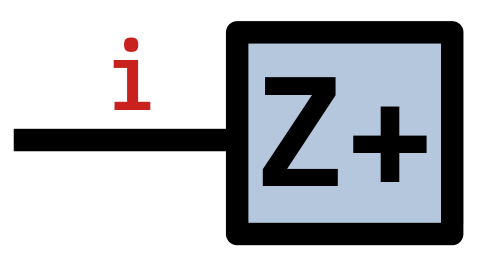
\includegraphics[width=0.3\textwidth]{
  slides/assets/Zp.png
} \\
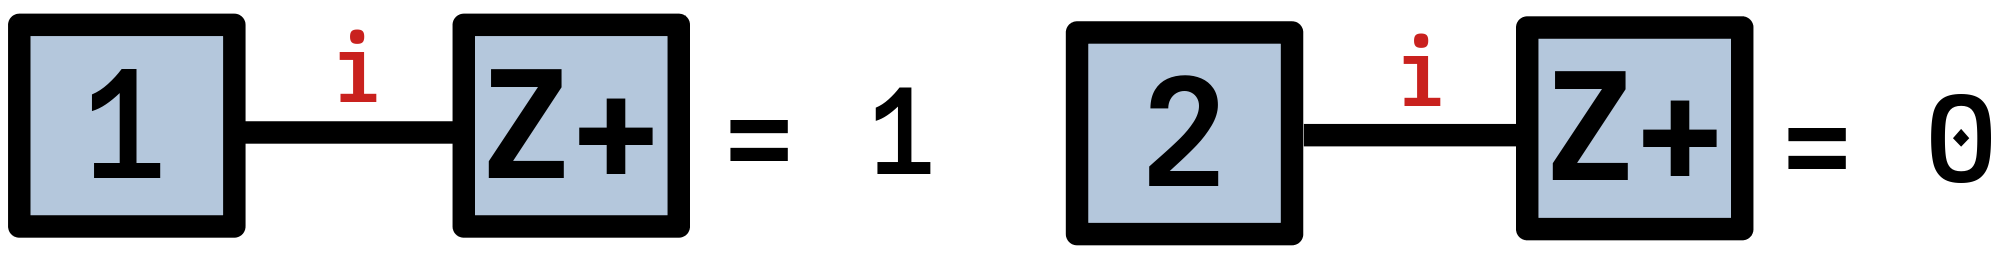
\includegraphics[width=1.0\textwidth]{
  slides/assets/Zp_elts.png
}
\end{center}
\end{onlyenv}
\end{column}

\end{columns}

\end{frame}
